\documentclass{article}[10pt, letter]
\usepackage{graphicx}
\usepackage{mathpazo}
\usepackage{amsmath}
\usepackage{amssymb}
\usepackage{endnotes}
\graphicspath{{./figs.}}

\title{Lattice Theory of Information}
\author{C.E. Shannon\thanks{Annotations, notes, and figures: \\ Hans Riess \\ University of Pennsylvania \\Department of Electrical/Systems Engineering \\ \texttt{hmr@seas.upenn.edu}}}
\date{}

\begin{document}


\maketitle

\begin{abstract}
	The word ``information" has been given many different meanings by various writers in the general field of information theory. It is likely that at
	least a number of these will prove sufficiently useful in certain applications to deserve further study and permanent recognition. It is hardly to be
	expected that a single concept of information would satisfactorily account for the numerous possible applications of this general field. The present note outlines a new approach to information theory which is aimed specifically at the analysis of certain communication problems in which there exist a number of information sources simultaneously in operation. A typical example is that 	of a simple communication channel with a path from the receiving point to the transmitting point. The problem is to make use of the feedback information for improving forward transmission, and to determine the forward channel capacity when the best possible use is made of this feedback information. Another more general problem is that of a communication system consisting of a large number of transmitting and receiving points with some type of interconnecting network between the various points. The problem here is to formulate the best systems design whereby, in some sense, the best overall use of the available facilities is made.\endnote{The problem Shannon describes is referred to as the \textit{network coding} problem. The challenge is to increase the throughput of a network, that is the flow of information from any given soure to sink, without increasing the network capacity.} While the analysis sketched	here has not yet proceeded to the point of a complete solution of these	problems, partial answers have been found and it is believed that a complete	solution may be possible.
\end{abstract}

\section{The Nature of Information}

In communication theory we consider information to be produced by a suitable stochastic process. We consider here only the discrete case; the
successive symbols of the message are chosen from a finite ``alphabet" and it is assumed for mathematical simplicity that the stochastic process producing
the message has only a finite number of possible internal states. The message itself is then a discrete time series which is one sample from the
ensemble of possible messages that might have been produced by the information source. The entropy\endnote{\textit{Entropy} is the minimal number of bits required to represent a piece of information. Suppose $x$ is a discrete random variable with alphabet $\mathcal{A}$, and $x$ is drawn from the discrete distribution $p = (p_i)_{i \in \mathcal{A}}$ with $p_i = \mathbb{P}(x = i)$. Then, $$H(x) = -\sum_{i \in \mathcal{A}} p_i \log p_i.$$ Suppose $x$ is an ``information source" or "stochastic process"  which is what Shannon means by a random sequence $x \in \mathcal{A}^\omega$ where $\mathcal{A}$ is an alphabet (e.g. $\{0,1\}$). He assumes that each $x_n$ is generated by a distribution $$p_i(n) = \mathbb{P}(x_n = i)$$ where $i \in \mathcal{A}$ is a letter in the alphabet generated at the $n$th iteration . The entropy of source $x$ is the quantity $$H(x) = \lim_{n \to \infty} -\frac{1}{n}\sum_{i \in \mathcal{A}} p_i(1)p_i(2) \cdots p_i(n)\log \left( p_i(1)p_i(2) \cdots p_i(n)\right).$$} $H(x)$ of such a source is a measure of the amount of
information produced by the source per letter of message. However, $H(x)$ can hardly be said to represent the actual information. Thus, two entirely
different sources might produce information at the same rate (same $H$) but certainly they are not producing the same information.

To define a concept of actual information, consider the following situation. Suppose a source is producing, say, English text. This may be translated or encoded into many other forms (e.g. Morse code) in such a way that it is possible to decode and recover the original. For most purposes of communication, any of these forms is equally good and may be considered to contain the same information. Given any particular encoded form, any of the others may be obtained, (although of course it may require an involved computation to do so). Thus we are led to define the actual information of a stochastic process as that which is common to all stochastic processes which may be obtained from the original by reversible encoding operations. It is desirable from a practical standpoint and mathematically convenient to limit the kind of all allowed encoding operations in certain ways. In particular, it is desirable to require that the encoding operations be done by a transducer\endnote{According to \textit{Wikipedia}, a transducer is a general term for any device that converts energy from one form to another. Common examples include sensors (responding to stimulus from a physical system) and actuators (devices that stimulate a physical system). Some devices such as radio antennae are both sensors and actuators.} with a finite number of possible internal states. This finite memory condition prevents paradoxical situations in which information goes into a transducer more rapidly on the average than it comes out at the output.

Each encoded version of the original process may be called a \textit{translation} of the original language. These translations may be viewed as different ways of describing the same information in about the same way that a vector may be described by its components in various coordinate systems.\endnote{Shannon is comparing a particular translation of a data stream to a change of basis of a finite dimensional vector space.} The information itself may be regarded as the equivalence class of all translations or ways of describing the same information.\endnote{Shannon is making the point that information is not a set of stochastic processes itself, but an set of equivalence classes of stochastic processes up to translation. He implicitly defines the following equivalence relation: $x \sim y$ if $y$ is a reversible translation of $x$, or vice versa.}

\section{The Metric, Topology and Convergent Sequences}

With this definition of information, it is possible to set up a metric\endnote{Recall, a metric space $(M,\rho)$ is a set $M$ with a binary function $\rho: M \times M \to \mathbb{R}_{+}$ satisfying i) $\rho(x,y) = 0$ if and only if $x = y$, ii) $\rho(x,y) = \rho(y,x)$, and iii) $\rho(x,y) + \rho(y,z) \leq \rho(x,z)$ (Triangle Inequality).} satisfying the usual requirements. The metric $\rho(x,y)$ measures the distance between two information elements $x$ and $y$, and is given in terms of conditional entropies.\endnote{Now, $H(x \vert y)$ is more common notation for Shannon's $H_y(x)$.}
We define
\[
\rho(x, y) = H_x(y) + H_y(x) = 2 H(x,y) - H(x) - H(y).
\]
The symmetry property $\rho(x,y) = \rho(y,x)$ is obvious from the definition. If $\rho(x,y) = 0$, both $H_x(y)$ and $H_y(x)$ must be zero (since both are necessarily non-negative), and this requires that the $x$ sequence be calculable with probability $1$ from the $y$ sequence and vice versa. The triangle law for the metric
\[
\rho(x,y)  + \rho(y,z) \geq \rho(x,z)
\]
is readily shown by expanding these terms into various entropies and making use of known inequalities for entropies. It may be noted that $\rho(x,y)$ is independent of the particular translations of $x$ and $y$ used in its calculation. This is due to the fact that $H_x(y)$ and $H_y(x)$ are invariant under finite state encoding operations applied to $x$ and $y$.

The existence of a natural metric enables us to define a topology for a set of information elements and in particular the notion of sequences of such elements which approach a limit.\endnote{Recall, a \textit{topology} on a set $X$ consists of a collection of open sets $\mathcal{U} = \{U_\alpha\}_{\alpha}$ such that an arbitrary union of sets in $\mathcal{U}$ is in $\mathcal{U}$ and a finite intersection of sets in $\mathcal{U}$ is in $\mathcal{U}$. Metric spaces are endowed with the \textit{metric space topology}; this topology is generated by taking arbitrary unions and finite intersections of sets of the form $B_{\epsilon}(x) = \{y \in M: \rho(x,y) < \epsilon\}$ called \textit{balls}. Open sets (i.e.~a topology) is enough data to define a notion of convergent sequences.} A set of information elements $x_1, x_2, \dots, x_n, \dots$ will be said to be Cauchy convergent if 
\[
\lim_{m \to \infty} \rho(x_m,x_n) = 0.
\]
The information of these sequences as new elements (analogous to irrational numbers) completes the space in a satisfactory way and enables one to simplify the statement of various results.\endnote{In a metric space, a \textit{Cauchy} sequence is a sequence $x_n$ that satisfies the property aforementioned. Shannon is referring to the process of completing a metric space by adding just enough points until every Cauchy sequence converges; a metric space in which every Cauchy sequence converges is called \textit{complete}. He reminds the reader that the real numbers are a completion of the rational numbers by adding ``irrational" numbers.}

\section{The Information Lattices}

A relation of inclusion\endnote{Shannon goes on to explain that this ``relation of inclusion" is a \textit{partial order}. A set $P$ is a partial order $(P, \leqslant)$ if it satisfies the following properties: i) $x \leqslant x$ for all $x$, ii) $x \leqslant y$ and $y \leqslant z$ imply $x = y$, and iii) $x \leqslant y$, $y \leqslant z$ imply $x \leqslant z$.} $x \geqslant y$, between two information elements $x$ and $y$ can be defined by
\[
x \geqslant y \quad \textrm{if and only if} \quad H_x(y) = 0.
\]
This essentially requires that $y$ be obtained by a suitable finite state operation\endnote{Shannon may mean that there is an finite state automaton that has $x$ as an initial state and $y$ as an accepting state.} (or limit of such operations) on $x$. If $x \geqslant y$ we call $y$ an \textit{abstraction} of $x$. If $x \geqslant y$, $y \geqslant z$, then $x \geqslant z$. If $x \geqslant y$, then $H(x) \geq H(y)$.\endnote{We would say that $H$ is an order-preserving map (also known as a monotone or isotone map) between the set of information elements and the positive real numbers.} Also $x > y$ means $x \geqslant y$, $x \neq y$. The information element, one of whose translations is the process which always produces the same symbol, is the $0$ element, and $x \geqslant 0$ for any $x$.

The \textit{sum}\endnote{In modern-day notation,  we would say that $z$ is the \textit{join} of $x$ and $y$ and write $z = x \vee y$.} of two information elments, $z = x + y$, is the process one of whose translations consists of the ordered pairs $(x_n, y_n)$ where $x_n$ is the $n$th symbol produced by the $x$ sequence and similarly for $y_n$. We have $z \geqslant x$, $z \geqslant y$ and there is no $w < z$ with these properties; $z$ is the least upper bound of $x$ and $y$. The element $z$ represents the total information of both $x$ and $y$.

The \textit{product}\endnote{Likewise, we would say that $z$ is the \textit{meet} of $x$ and $y$ and write $x \wedge y$. With this terminology, a \textit{lattice} is a partial order such that $x \vee y$ and $x \wedge y$ exist for all $x$ and $y$. Equivalently, a lattice is a set $L$ with two binary operations $\vee$ and $\wedge$ satisfying a set of axioms. What are they?} $z = x y$ is defined as the largest $z$ such that $z \leqslant x$, $z \leqslant y$; that is, there is no $w > z$ which is any abstraction of both $x$ and $y$. The product is unique. Here $z$ is the common information of $x$ and $y$.

With these definitions a set of information elements with all their sums and products forms a metric lattice. The lattices obtained in this way are not, in general, distributive, or even modular.\endnote{Shannon is referring to two important properties of lattices. A lattice is distributive if $x \wedge (y \vee z) = (x \wedge y) \vee (x \wedge z)$ and $x \vee (y \wedge z) = (x \vee y) \wedge (x \vee z)$ for all $z$. For instance, the collection of subsets of a set is a lattice with unions and intersections; this lattice is distributive. A lattice is modular if it obeys the law: $x \leqslant y$ implies $x \vee (y \wedge z) = (x \vee z) \wedge y$. For instance, the collection of subspaces of a vector space is a modular lattice.} However they can be made to be relatively complemented by the addition of suitable elements. For $x \leqslant y$ it is possible to construct an element $z$ with
\begin{align*}
	z + x = y \\
	z x = 0.
\end{align*}
The element $z$ is not, in general, unique.

The lattices obtained from a finite set of information sources are of a rather general type; they are at least as general as the class of finite partition lattices. With any finite partition lattice it is possible to construct an information lattice which is abstractly isomorphic by a simple procedure.\endnote{This claim Shannon states without proof. Let's try to provide some context. Let $\Pi(m)$ be the lattice of partitions of a finite set $\{1,2, \dots, m\}$. $\Pi(m)$ is a lattice under the refinement order: $\pi \geqslant \rho$ if $\pi$ is a refinement of $\rho$. Intuitively, $\pi$ contains more information than $\rho$. Without loss of generality, suppose $\mathcal{A} = \{0,1, \dots, m\}$ is our alphabet. Every partition $\pi$ is in one-to-one correspondence with an equivalence relation on $\{1,2, \dots, m\}$. Suppose $\pi$ contains $k$ -many equivalence classes. For each equivalence class $[x] \in \pi$, let $p_i(n) = 1/(k \cdot \#[x])$ and let $x$ be the information element given defined by the join distribution $p_i = (p_i(1), p_i(2), \dots, p_i(n))$ for each $n$. This procedure may be what Shannon had in mind for defining an isomorphism between partition lattices and a corresponding lattice of information.} 

\noindent Some example of simple information lattices are shown in Figs.~\ref{fig:1} and \ref{fig:2}.

In Fig.~\ref{fig:1}, there are three independent sources. The product of any two of these elements is zero, and the conventional lattice diagram\endnote{The ``conventional lattice diagram" he refers to is a \textit{Hasse diagram} of a partial order. In a Hasse diagram, elements $x$ and $y$ of a lattice are connected by an edge if $y$ covers $x$ written $x \prec y$ meaning that $x < y$ and there is no $z$ such that $x < z < Y$.} is that shown at the right. In Fig.~\ref{fig:2}, there are two independent sources of binary digits, $x$ and $y$. The sequence $z6$ is the sum modulo $2$ of corresponding symbols from $x$ and $y$. In this case again the product of any two of $x$, $y$ and $z$ is zero, but the sum of any two represents the total information in the system. In this case the lattice is non-distributive, since $z y + z x = 0 + 0 = 0$, while $z (x+y) = z \neq 0$.

\begin{figure}
	\begin{center}
		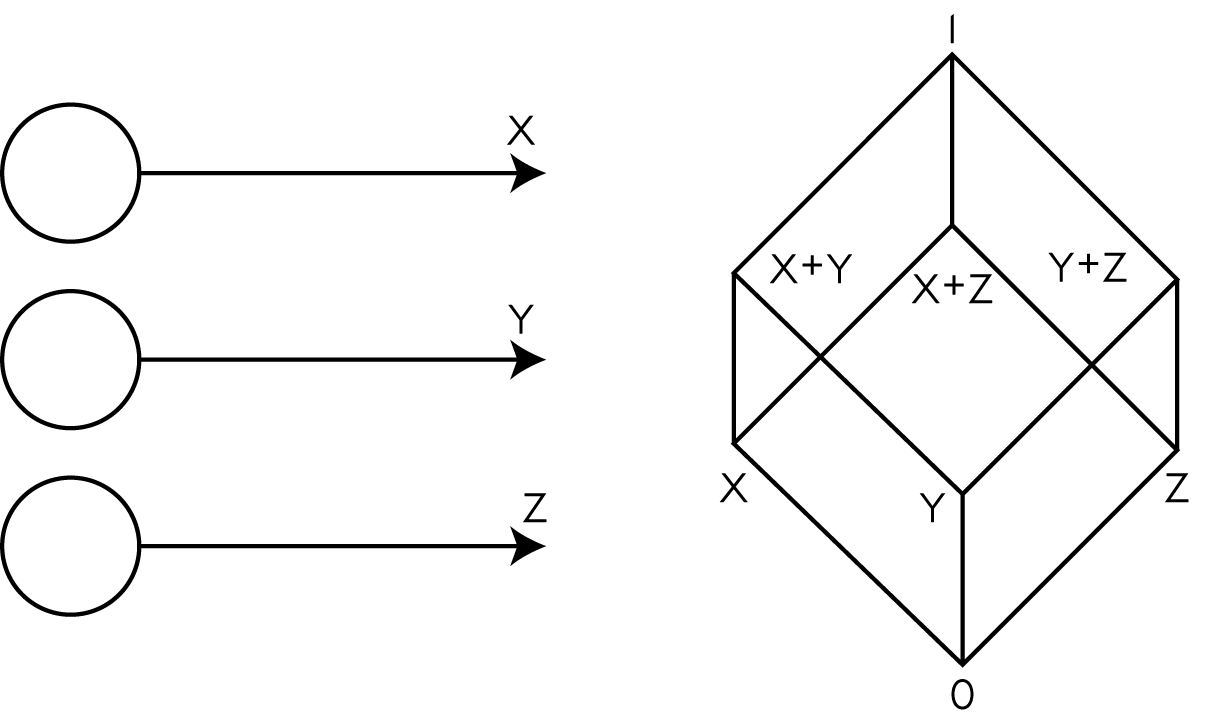
\includegraphics[width=0.5\textwidth]{fig1}
		\end{center}
	\caption{}\label{fig:1}
\end{figure}

\begin{figure}
	\begin{center}
		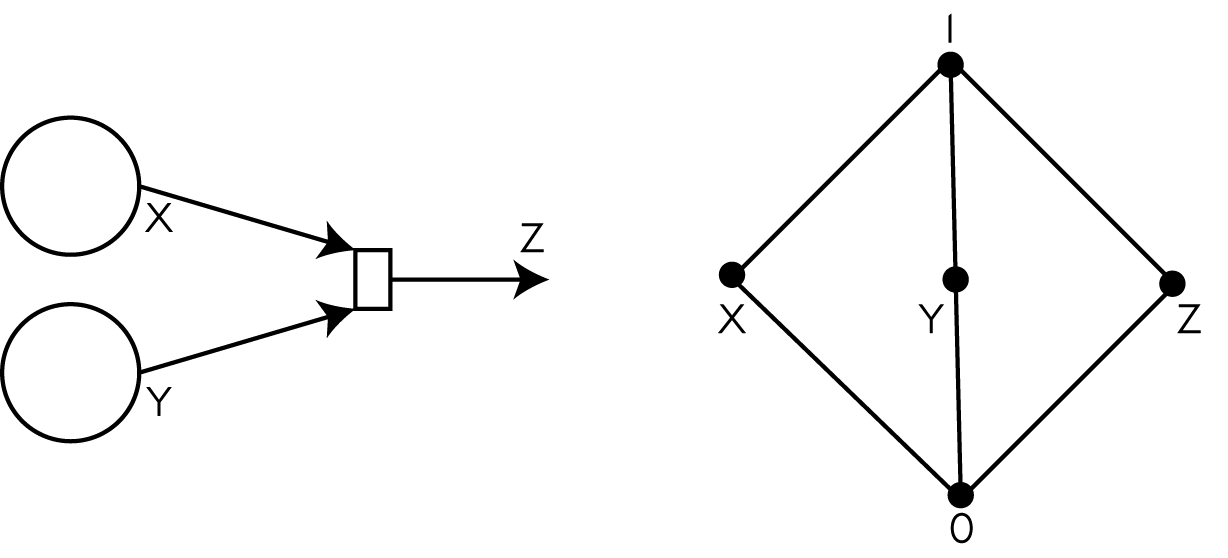
\includegraphics[width=0.5\textwidth]{fig2}
	\end{center}
	\caption{}\label{fig:2}
\end{figure}
	


\section{The Delay Free Group $G_1$}

The definition of equality for information based on the group\endnote{A \textit{group} is a set $G$ with a binary operation $\star: G \times G \to G$ satisfying the following conditions: i) $g \star (h \star k) = (g \star h) \star k$, ii) there exist a unique element $e \in G$ such that $g \star e = e \star g = g$ for all $g \in G$, iii) for every $g \in G$ there is a unique element called $g^{-1}$ such that $g \star g^{-1} = g^{-1} \star g = e$. Reversible encoding operations form a group: encodings can be composed by applying them one after another, every reversible has an inverse decoding, and the null encoding (do nothing) is the identity element.} $G$ of all reversible encoding operations allows $x = y$ when $y$ is, for example, a delayed version of $x$; $y_n = x_{n+a}$. In some situations, when one must act on information at a certain time, a delay is not permissible. In such a case we may consider the more restricted group $G_1$ of \textit{instantaneously reversible} translations. One may define inclusion, sum, product, etc., in an analogous way, and this also leads to a lattice but of much greater complexity and with many different invariants.

\theendnotes

\end{document}